\section{Der Roboter}

Diese Arbeit behandelt einen Roboterschwarm im zweidimensionalen Raum. Dabei hat sich der Autor für den 
R-One entschieden. Dieser besitzt 8 Infrarot-Sensoren zur Ermittlung von Nachbarn, zwei Räder um sich
auf dem Boden fortzubewegen, einen Prozessor, Speicher und Batterie. Da die Infrarot-Sensoren ab einem
Meter stark an Genauigkeit abnehmen werden die Roboter einen Abstand von weniger als einen Meter einhalten.
Die Sensoren eines Roboters $R_i$ teilen nun den umliegenden Raum in 16 Teile auf, um die Nachbarn anhand 
ihrer Lage und Ausrichtung zu $R_i$ zu speichern. In der Abbildung sieht man, wie die Sensoren den Raum
aufteilen. Nachbarn eines Roboters $R_i$ werden nun nach folgender Formel gespeichert:\\

$q_j^i=(x_j^i,y_j^i,\theta_j^i)=(d_{ij}\cos(b_j^i),d_{ij}\sin(b_j^i),b_j^i+\pi-o_j^i)$\\\\
Diese Formel speichert die Koordinaten und Ausrichtung eines Nachbarn, ausgehend von $R_i$ als Ursprung
eines Koordinatensystems. $x$ und $y$ bilden dabei die Koordinaten im Raum und $\theta$ die Ausrichtung.
Man kann die Position eines Nachbarn auch durch $d$, $b$ und $o$ speichern, wobei diese Formel einen Kreis
um $R_i$ mit Radius $d$ zieht, der Nachbar dann an der Stelle $b$ auf dem Kreis liegt und $o$ die
Ausrichtung zu $R_i$ angibt. Im zweiten Verfahren werden alle Werte in Grad gemessen. Die Ausrichtung eines
Nachbarn zu $R_i$ ermittelt sich übrigens daraus, welche Sensoren ausgehend vom "Kopf" des Roboters
angesprochen werden, und die Roboter so den Winkel der Ausrichtung durch Abgleichen der ID ihrer Sensoren
erkennen.\\

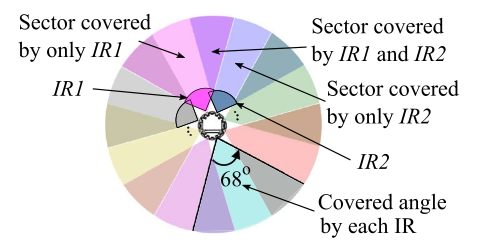
\includegraphics[width=3in]{images/Screenshot 2023-02-16 at 11.53.03 AM.png}\\\\
Die Roboter tauschen nun ständig im Millisekundentakt ihre Nachbarn aus und speichern diese als Array.
Als nächstes betrachten wir, wie mehrere solcher Roboter einen Schwarm bilden.